\documentclass[10pt,letterpaper]{article}
\usepackage{amsmath}
\usepackage{amsfonts}
\usepackage{amssymb}
\usepackage[english]{babel}
\usepackage{breakurl}
\usepackage[superscript]{cite}
\usepackage{fancyhdr}
\usepackage{float}
\usepackage[margin=1in]{geometry}
\usepackage{graphicx}
\usepackage{hyperref}
\usepackage[utf8]{inputenc}
\usepackage{makeidx}
\usepackage{multicol}
\usepackage{nth}
\usepackage{longtable}

% Use Helvetica
\usepackage[scaled]{helvet}
\renewcommand\familydefault{\sfdefault} 
\usepackage[T1]{fontenc}

\usepackage{setspace}
\usepackage{siunitx}
\usepackage{svg}
\usepackage{subcaption}
\usepackage{tikz}
\usepackage{titling}
\usepackage{url}
\usepackage{kantlipsum}
\usepackage{enumitem}

\usepackage{parskip} % Paragraph skip - adds extra lineskip spacing
\setlength{\parskip}{0.7\baselineskip plus 2pt}

% Subsubsubsection
\usepackage{titlesec}
\setcounter{secnumdepth}{4}
\titleformat{\paragraph}
{\normalfont\normalsize\bfseries}{\theparagraph}{1em}{}
\titlespacing*{\paragraph}
{0pt}{3.25ex plus 1ex minus .2ex}{1.5ex plus .2ex}

% Custom definitions
\newcommand{\doctitle}{Design Document}
\newcommand{\docsubtitle}{Computing Platform Multirotor with FPGA Hardware Acceleration Applications}

% Custom commands
\newcommand{\ts}{\textsubscript}	% Subscript command %

% Use hyphans to break up urls
\def\UrlBreaks{\do\/\do-}

% PDF and href setup
% Hyper ref
\hypersetup{
	colorlinks=true,
	citecolor=black,
	linkcolor=black,
	filecolor=black,
	urlcolor=blue,
	pdftitle={\@title},
	bookmarks=true
}
\urlstyle{same}

% Page headings
\pagestyle{fancy}
\fancyhead[L]{\MakeUppercase{CPEN/ELEC 491}}
\fancyhead[R]{\textbf{Team 109}}
\fancyfoot{}
\fancyfoot[C]{\thepage}

% No paragraph indent
\parindent 0ex

% Meta
\author{
	Deutsch, Peter &
	\textit{me@peterdeutsch.ca}
	\\
	He, Muchen &
	\textit{i@muchen.ca}
	\\
	Hsueh, Arthur &
	\textit{ah11962@outlook.com}
	\\
	Wang, Meng &
	\textit{wzfftxwd@gmail.com}
	\\
	Wilson, Ardell &
	\textit{ardellw96@gmail.com}
}
\title{\doctitle}
\date{\today}

\makeatletter
\renewcommand{\maketitle}{
	\bgroup
	\setlength{\parindent}{0pt}
	\begin{flushleft}
		% Top spacing
		\vspace*{0.75in}

		% Team logo
		
\includegraphics[scale=0.5]{../assets/capstonelogo1.png}
		\vspace*{0.25in}

		% Title
		\textbf{\Huge{\@title}}\\
		\hrulefill

		% Subtitle
		\textbf{\huge{\docsubtitle}}
		
		\vspace*{0.5in}

		% Course number and team
		\textbf{\Large{CPEN/ELEC 491 Capstone Team 109}}\\
		\hspace*{0.1cm}
		\begin{tabular}[h]{|ll}
			\@author
		\end{tabular}

		\vspace*{0.25in}

		\textbf{Website}: https://capstone-skynet.github.io

		\vfill

		% Logo
		\hspace*{-0.3cm}
\includegraphics[scale=0.5]{../assets/ece_logo.pdf}

		% Date
		\large{\@date}
	\end{flushleft}
	\egroup
}
\makeatother

% Begin Document
\begin{document}

% Title Page
\begin{titlepage}
	\maketitle
\end{titlepage}

% Executive Summary (Not used here in proposal)
% \include{executive_summary.tex}

% Revision history
%\thispagestyle{empty}
\section*{Revision History}
The full revision history and commited changes of the document can be found in the git repository history: \href{https://github.com/Capstone-Skynet/Capstone-Skynet.github.io}{https://github.com/Capstone-Skynet/Capstone-Skynet.github.io/commits/master}.

\begin{table}[H]
\begin{tabular}{*{4}{l}p{0.5\linewidth}}
\hline
Version \# & Initials & Release Date & Changeset & Changes Made \\ \hline

0.0 & PD & 2019-10-11 & \texttt{660e001} & Initial skeleton of the document.\\
0.1 & MH & 2019-10-11 & \texttt{6af9e8a} & Populate initial document with draft content required for Milestone I.\\
0.2 & PD & 2019-11-23 & & Initial framework for test descriptions created.\\
0.3 & MW & 2019-11-24 & & First set of tests added.\\
1.0 & PD & 2019-11-25 & & General clean-up and release for Milestone II.\\
1.1 & AH & 2020-02-09 & & Added Full System Tests \\

 & & & \\ \hline
\end{tabular}
\end{table}

% Table of contents
\setcounter{secnumdepth}{3}
\tableofcontents

% Terms and Abbreviations
\thispagestyle{empty}

\section*{Terms and Abbreviations}

Technical terms and abbreviations dictionary go here.

\begin{tabular}[h]{rp{0.75\linewidth}}
    \hline
    \textbf{Term} & \textbf{Definition}\\
    \hline

    ANN & Artificial Neural Network, or simply ``Neural Network'', is a data processing model modeled after neuron interactions. The process consists of forward propagation using several matrix multiplications.\cite{ann}\\
    ASIC & Application-specific Integrated Circuits.\\
    CNN & Convolutional neural network are neural networks that is especially useful for image classification.\cite{cnn} \\
    ECE & Department of Electrical and Computer Engineering at the University of British Columbia.\\
    FPGA & Field-Programmable-Gate-Arrays, ``programmable'' hardware that allows ASIC-like performance with software-like turn-around time and flexibility.\\
    GPU & Graphics Processing Unit, a discrete piece of hardware designed to accelerate graphic-intensive or other parallel computing tasks.\\
    LOS & Line-of-sight.\\
    ML & Machine learning.\\
    Multirotor & An unmanned vehicle with multiple engines. \\
    OTS & Off-the-shelf, or commercially available/purchasable \\
    PID / PID Controller & Proportion-Integral-Derivative controllers is the most common control algorithm for precise and accurate movement, as well as to compensate external forces.\cite{pid}\\
    RNN & Recurrent neural networks are neural networks where the output depends on previous computations, essentially consists of memory.\cite{rnn}\\
    RX & Receiver.\\
    TC & Transport Canada.\\
    TX & Transmitter.\\
    YOLO & You-Only-Look-Once is a fast ML algorithm that detect objects but is unlike CNN nor RNN.\cite{yolo}\cite{yolo-2}\\
     & \\

    \hline

\end{tabular}


% List of figures and tables
\thispagestyle{empty}
\listoffigures
\listoftables
\newpage

% Set page and section counter
\setcounter{page}{1}

% TODO: fill out all the sections
% if the sections gets too long, move them to a separte .tex document
\section{About This Document}
This document will contain a concise description of the design decisions made during the project.

\subsection{Purpose}

\subsection{Intended Audience}

\subsection{Reading Guide}

\section{High Level Design}\label{high_level_design}
\subsection{Overview}
The device is composed of two distinct systems, the \textit{Computing Platform} and the \textit{Multirotor}, which work in tandem to capture aerial video, analyze it through hardware-accelerated processes, and convey the results of the analysis to the end-user. 

\begin{figure}[H]\label{hlpic}
    \centering
    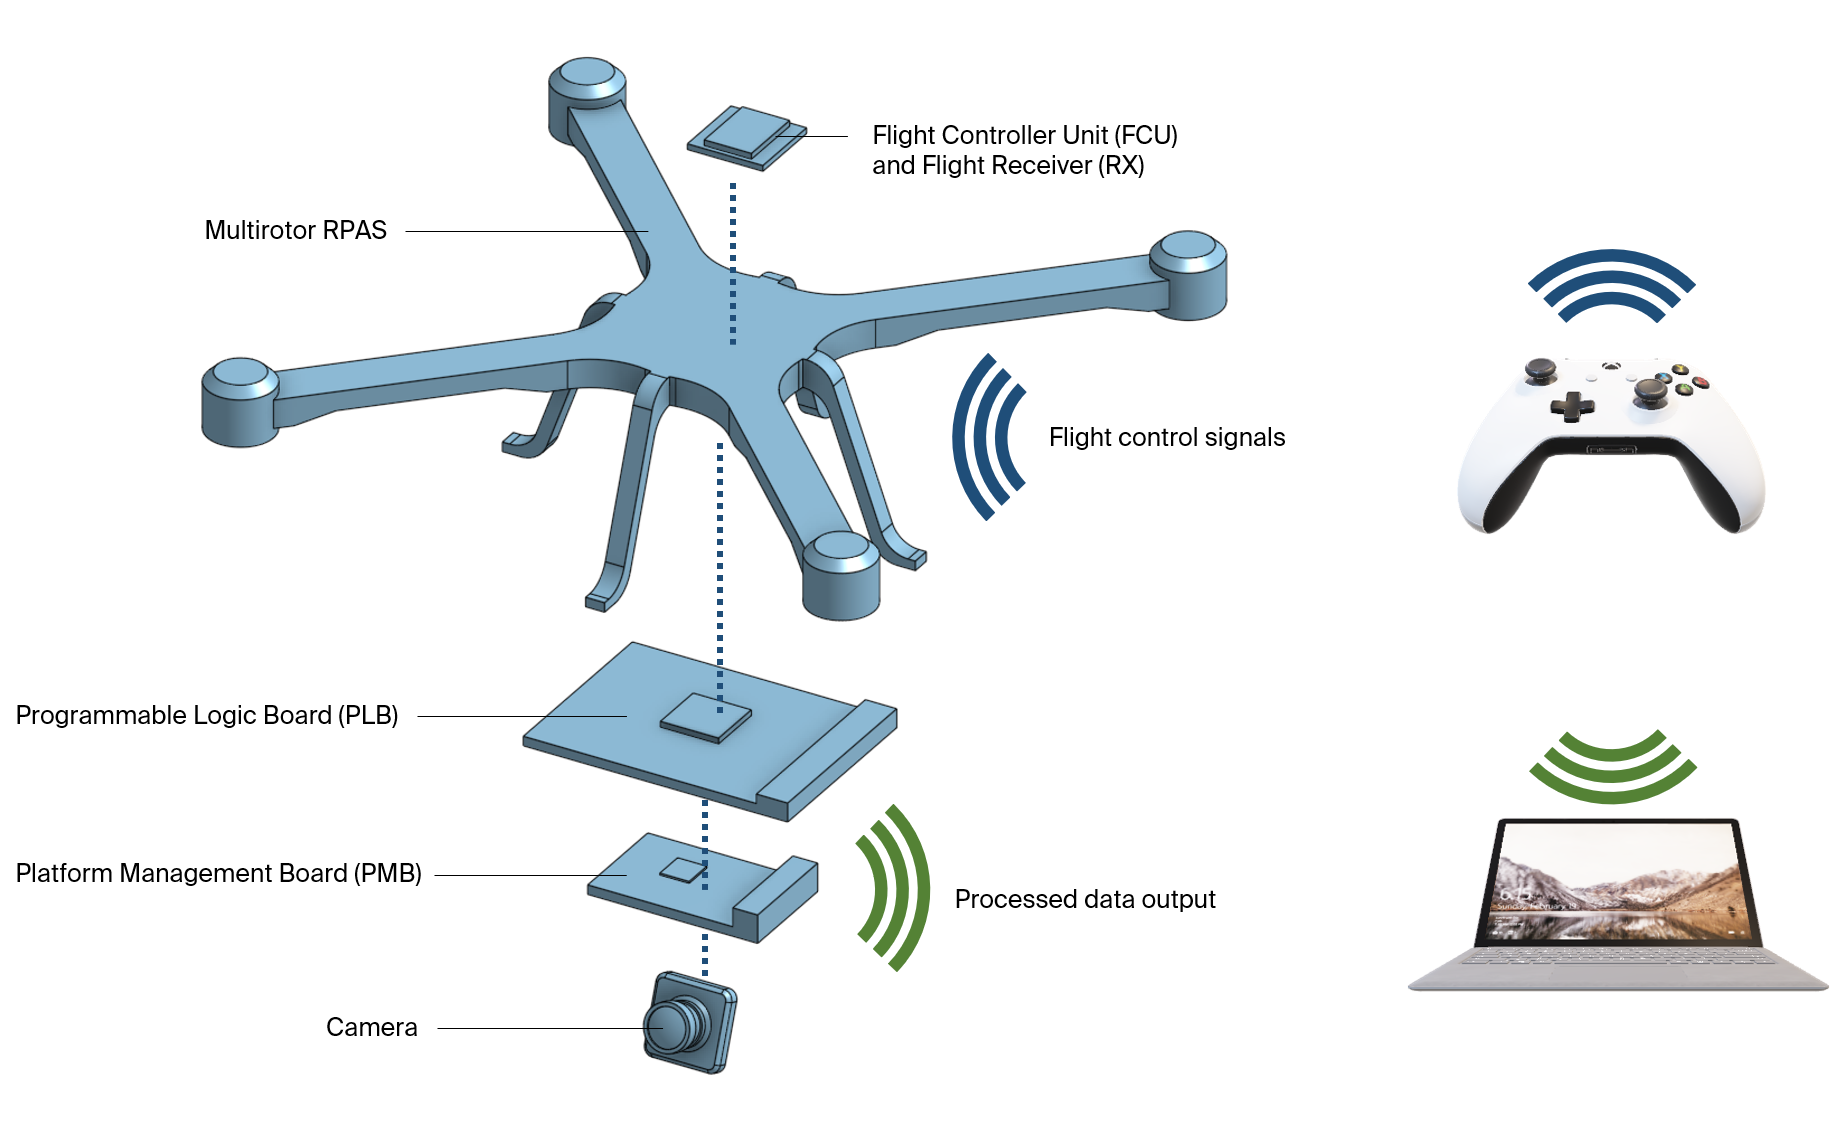
\includegraphics[width=\linewidth]{img/intpic.png}
\caption{High-Level System Integration with RPAS}
\end{figure}

\textbf{The \textit{Computing Platform}} is comprised of three processing platforms: the \textit{Platform Management Board} (PMB), the \textit{Programmable Logic Board} (PLB), and the \textit{Base Station}. The \textit{PMB} and \textit{PLB} are mounted to the multirotor, while the base station is a mobile device utilized by the user at ground-level.

The \textit{Platform Management Board} (a Raspberry Pi 4) is responsible for managing the majority of the aerial computations and communications. This includes managing video acquisition, conveying data to and from the PLB to facilitate hardware accelerated machine learning tasks, and transmitting video and ML results to the base station via a WiFi connection.

The \textit{Programmable Logic Board} (a Digilent Zedboard), connected to the PMB via Ethernet, facilitates the hardware-acceleration functionalities of the device. It is comprised of a hard-processor (ARM Cortex A9) and an FPGA interfaced via an on-chip interconnect. The FPGA hosts the hardware acceleration unit, which is (currently) driven by a YOLOv2 open-source accelerator IP core. As this device is intended to act as an experimental research platform, the client may replace this hardware accelerator with their own implementation upon delivery.

The \textit{Base Station} (a consumer laptop) connects to the multirotor via WiFi, displaying live video and ML results as transmitted by the aerial computing components. In addition to conveying the video and ML analytics, the base station also provides remote control of the computing system -- allowing the user to monitor system status and alter parameters of ongoing computations on-the-fly.

\textbf{The \textit{Multirotor}} is a quad-engine remote-piloted-aerial system, or multirotor/quadcopter RPAS for short.
The RPAS is propelled electrically using DC sources and motors, controlled by an onboard flight controller unit (FCU) that samples accelerometer data to make fine adjustments to the flight kinematics.
The RPAS is equipped with a receiver to enable flight control via standard radio-control (RC, 2.4 GHz) by a pilot.

The RPAS and computing platform are relatively independent as the computing platform provides its own power source. The two modules impose constraints on each other: the computing platform (including its power source) must be light and compact such that it can be lifted by the RPAS. 
Likewise, the RPAS must provide mounting mechanisms for the computing platform and provide clearance such that equipment is not damaged during flight operations.

\subsection{System Data Flow}

\begin{figure}[H]
\centering
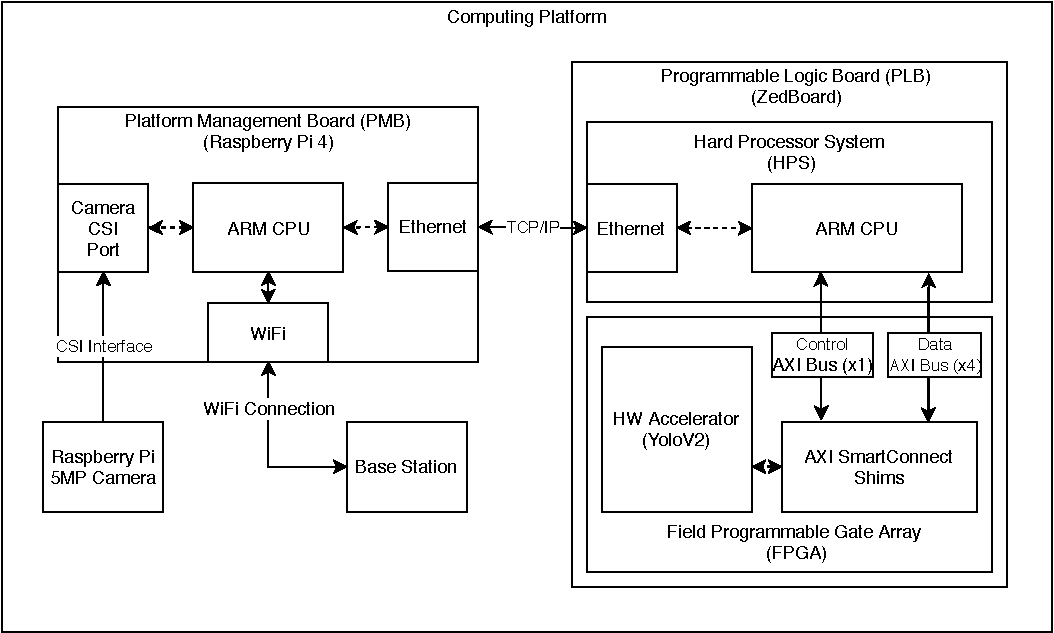
\includegraphics[width=15cm]{img/pc_diagram.pdf}
\caption{High-Level System Architecture}
\label{pcdiag}
\end{figure}

A step-by-step overview of the data flow within the computing platform (seen in Figure \ref{pcdiag}) is as follows:
\begin{enumerate}
\item The on-board camera captures a video frame and transmits it to the PMB via a CSI interface
\item The PMB sends the video frame to two locations:
\begin{enumerate}
\item The PLB, via a TCP/IP Ethernet link, to perform hardware-accelerated machine learning, and
\item The base station, via a TCP/IP WiFi link, to display to the end-user
\end{enumerate}
\item The ARM core on the PLB receives the video frame from the PMB via the ethernet link, further processes it, and dispatches hardware acceleration requests to the FPGA portion via parallel AXI buses
\item The FPGA portion receives the video frame (which first passes through AXI shims to facilitate clock synchronization) and processes this frame within the hardware acceleration core
\item Upon completion, the hardware acceleration core sends machine learning results back to the ARM core, which itself transmits the data back to the PMB via the Ethernet link
\item The machine learning results are transmitted over the WiFi link to the base station
\item The base station overlays the video feed and machine learning results, displaying them on-screen
\end{enumerate}

Simultaneously, the user independently controls the operation of the multirotor through a standard radio controller, as described in Section \ref{multirotor}.

\section{Technical Subsystems Design}\label{technical_design}

\subsection{Computing Platform}\label{computing_platform}

\subsubsection{Video Capture}\label{video_capture}
% TODO: Talk about camera choice, MIPI interface, camera libraries. Also, talk about alternatives we explored (i.e. analog video transmission/acquisition.

\subsubsection{Subsystem Overview}
The video capture subsystem of the computing platform consists of a camera, the video transmission protocol to the processing core, and video transmission to the base station. For this subsystem, the hardware utilized includes a CMOS camera, a Raspberry Pi device, and a MIPI Camera Serial interface. 

\subsubsection{Camera Choice}
The camera used to capture video is the \textit{Raspberry Pi Camera Module}. This module supports 1080p, 720p and 480p video, captured using a fixed focus lens. The camera captures live video and sends it to the PMB, which feeds the data to both the machine learning model and the base station.

A major consideration regarding camera selection was the latency and throughput of the machine learning implementation on the FPGA. As the machine learning implementation is heavily constrained by the FPGA's limited resources, it is not necessary to use a camera with a high resolution and framerate.

% {MIPI interface}
\subsubsection{MIPI Interface and Libraries}
The MIPI camera serial interface (CSI) is a high-speed protocol primarily intended for point-to-point image and video transmission between cameras and host devices. 

The MIPI protocol has been widely adopted for image and video transmission, and as such the camera can easily be replaced by the client in the future, if desired (fulfilling constraint \textbf{C.EX.5}).

% {Camera libraries or getting the video to a 'viewable' state}
Live video acquisition is managed through the utilization of the open-source 'raspicam' C++ library. Facilitating image/video capture, 'raspicam' was selected over the native Raspberry Pi camera libraries in order to perform capture and processing in a low-level C++ environment. This allows for required low-level memory manipulation/image format conversions to be performed directly on the (more powerful) PMB, rather than the PLB.

% {Explored Alternatives}
\subsubsection{Explored Hardware Alternatives}
There were many alternatives explored for each component of the video capture subsystem.

One of the possibilities explored for the camera subsystem was the purchase of a drone package with a pre-integrated camera. The implicit requirement to disassemble and reconfigure/tap-into a hard-wired system, however, would create an unmaintainable product -- making user replacement of the camera for future research improvements difficult (violating constraint \textbf{C.EX.5}).

Another consideration for the subsystem involved utilizing a USB webcam -- connecting it via the Raspberry Pi's USB port. The issue with this option is the inferior configurability of the webcam compared to the Raspberry Pi camera. The reconfigurability provided by the 'picamera' Python package, as previously noted, made the Rasberry Pi Camera a better solution suited to the client's needs.

A possible alternative explored for the camera interface was RS-232. The RS-232 interface is a commonly used, easy to integrate serial interface. It is widely used in the communications area, however its low data transfer rate limits both the resolution and frame rate of the video footage that can be captured. The highest (reliable) baud rate of the RS-232 interface is approximately 115200 bits per second -- translating to a frame rate of 0.05 fps for 480p video footage (violating constraint \textbf{NF.CM.3}).

For the live video feed transmission, other options explored include wireless HDMI, VGA and analog transmission methods.  Ultimately these options required additional hardware (contributing to higher costs and system weight) and would introduce more points of failure and complexity into the finalized system, thus they were not pursued.


\subsubsection{Platform Management Board}\label{platform_management}
\subsubsection{Subsystem Overview}
The platform management board manages all I/O required by the computing platform: interfacing with the camera, programmable logic board (hosting the machine learning implementation), and base station. A separate system is used for the multirotor's flight control.

A decomposition of the system is seen in Figure \ref{pcdiag}.

\begin{figure}[H]
\centering
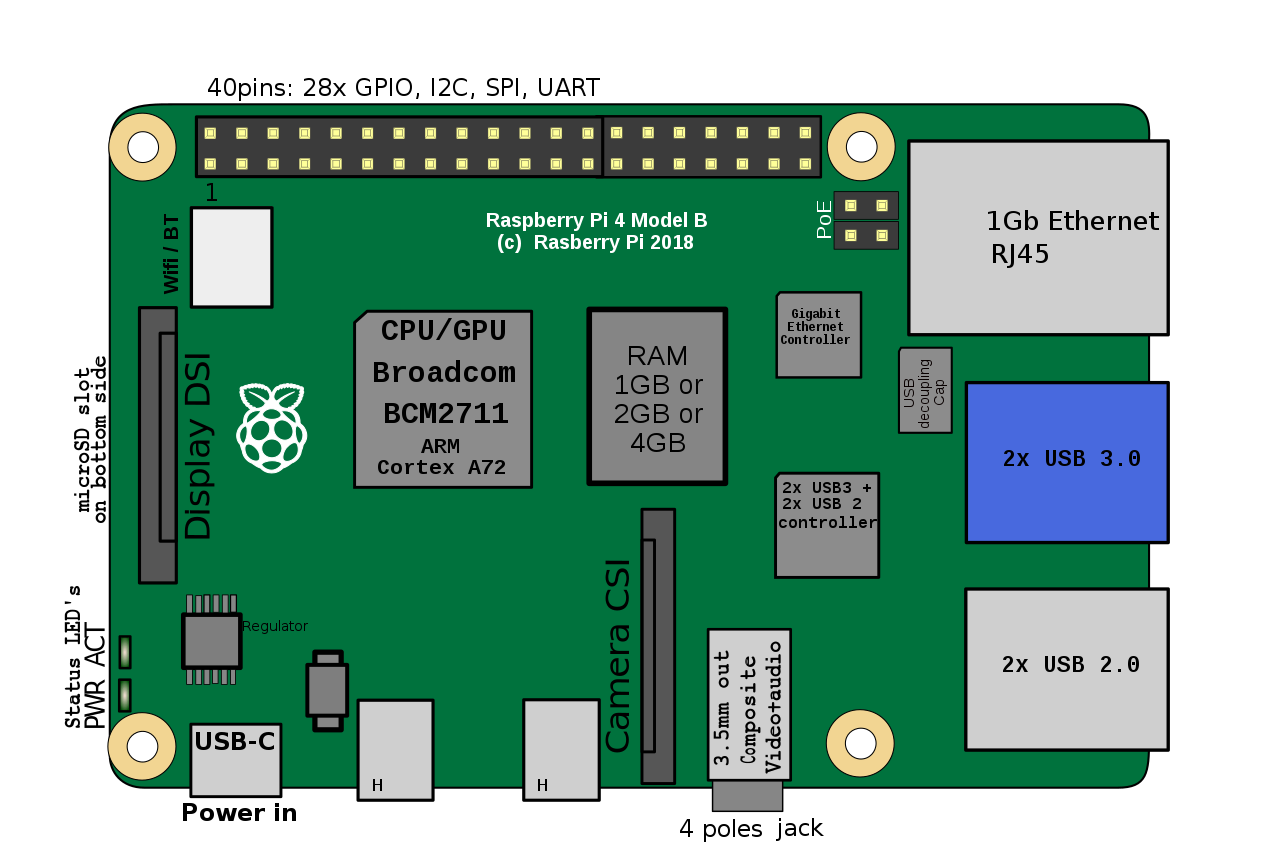
\includegraphics[width=10cm]{img/RaspberryPi_Model_4B.png}
\caption[Layout of Connectors and Main ICs on Raspberry Pi 4]{Layout of Connectors and Main ICs on Raspberry Pi 4\cite{rpidiag}}
\label{rpi}
\end{figure}

\subsubsection{Device Selection}
The selected device to implement the platform management system is the Raspberry Pi 4. As seen in Figure \ref{rpi}, the Raspberry Pi 4 is a small single-board computer that hosts a quad-core ARM Cortex A72 CPU, a CSI camera interface, 40 serial pins, Wi-Fi/Bluetooth, and a gigabit Ethernet port. We choose the Raspberry Pi 4 over other single-computer platforms (including Arduino/Beagleboard/Orange Pi) because the Raspberry Pi 4:
\begin{itemize}
\item is relatively inexpensive (CAN\$45 in November 2019),
\item has a large support community and a wealth of driver/library support,
\item supports a wide range of high throughput I/O standards (USB/WiFi/Ethernet/Serial, \textbf{C.EX.3}),
\item provides an industry-standard camera interface (\textbf{C.EX.5}),
\item supports extensible non-volatile storage (\textbf{F.CP.4}),
\item has been regularly succeeded with cross-compatible revisions (presumably, including the upcoming Raspberry Pi 5) --- therefore future-proofing the PMB segment,
\item has an established community for technical support, and
\end{itemize} 

\subsubsection{Data Flow}
The overall data flow managed by the Raspberry Pi is as follows:
\begin{enumerate}
\item Video is acquired through the camera CSI interface
\item Frame manipulation/correction is performed on the video, if required by the specific machine learning use-case
\item Manipulated video is decomposed and transmitted over Ethernet to the programmable logic board (which performs the machine learning)
\item Machine learning results are received via Ethernet
\item Video, ML results, and system status information are transmitted via WiFi to the base station
\item (Optional) Results and video are stored locally on non-volatile storage for post-flight analysis
\end{enumerate}

All operations are managed by the ARM Cortex A72 chip running a headless version of the Raspbian operating system. 

\subsubsection{Use of Multiple Computing Boards}
The presence of on-board WiFi/camera interfaces is the primary driving factor towards adopting a dual-board (Platform Management and Programmable) solution. While a single-board solution is possible, the development effort and cost of the computing platform would be considerably higher. Most programmable logic boards (including our chosen board, the Zedboard) require external expansion devices to interface with peripherals such as WiFi/cameras. These expansion devices, which connect to the programmable logic board via a serial connection, have poorly documented drivers and are of considerable expense -- ranging from US\$25 for a basic WiFi module\cite{digiwifi} to US\$200 for a compatible camera interface card\cite{digipmod}. External expansion devices also require considerable glue logic resources on the programmable logic board, potentially risking non-compliance with constraint \textbf{C.EX.2}.

An additional consideration in selecting the two-board design regards platform extensibility --- the client may desire to increase the programmable logic capabilities of the computing platform in the future, requiring a board swap. If a single-board solution is implemented, the client would be required to migrate \textit{all} hardware/software to the larger board, requiring them to devote considerable effort to debug driver issues. Additionally, external expansion devices are not necessarily compatible with all PLBs -- adding constraints to the client's board selection or requiring the purchase of new interface cards. By offloading the interfacing work to a distinct \textit{platform management} board, the client can easily replace the PLB without considerable redevelopment (fulfilling constraint \textbf{C.EX.4}). 

To emphasize, the use of multiple computing boards is a design decision derived from the requirement to use \textit{off-the-shelf} components in the development of this device. Upon the completion of new hardware-accelerated machine learning implementations, the client may wish to integrate the capabilities of both boards into a single (custom ASIC) platform. 

\subsubsection{Interface with Programmable Logic Board}

To interface with the PLB, data packets are sent via a bi-directional TCP/IP-managed Ethernet connection. TCP/IP over Ethernet was selected in lieu of serial solutions (such as I2C) as:
\begin{itemize}
\item Ethernet is equally as ubiquitous on modern programmable logic boards,
\item Ethernet has higher maximum throughput on modern platforms (on the Zedboard, 1 Gbps on Ethernet vs. 400 Kbps on serial)
\end{itemize} 

The selection of Ethernet over serial precludes the use of the \textit{Zero W} variant of the Raspberry Pi, as the Zero W does not provide Ethernet support. 


\subsubsection{Programmable Logic Board}\label{programmable_logic}
\subsubsection{Subsystem Overview}
 The PLB manages the hardware-accelerated ML application, performs additional pre/post-processing on ML data (if required by the ML application), and communicates with the platform management board.

A decomposition of the system is seen in Figure \ref{pcdiag}.

Of note is the distinction between the two portions present in the PLB: the Hard Processor System (HPS) and the FPGA. The Hard Processor System is a non-customizable CPU and is used for generic tasks such as managing I/O via the Ethernet port and processing non-acceleratable ML tasks. The FPGA provides the system's \textit{programmable circuity} -- performing the requisite hardware acceleration needed for ML tasks. The two systems co-reside on the same chip, and are interfaced via an internal bus.

\subsubsection{Device Selection}
The selected programmable logic board is the \textit{ZedBoard SoC Development Board} (pictured in Figure \ref{zedboard}), manufactured by Digilent. 

\begin{figure}
\centering
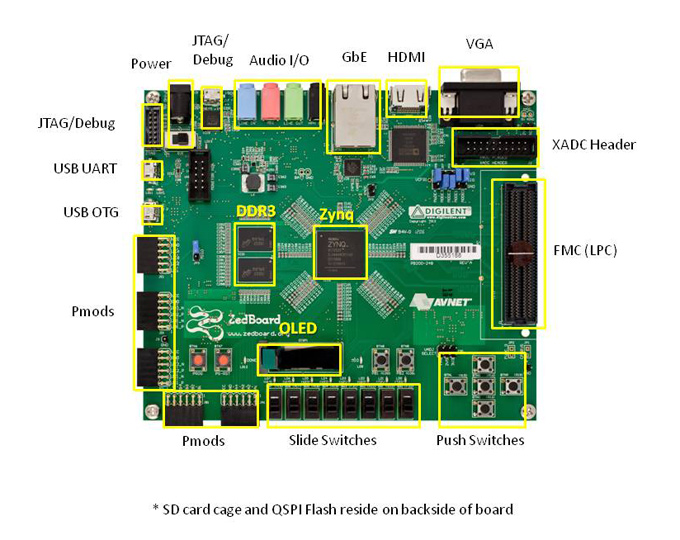
\includegraphics[width=12.5cm]{img/zedboard_functional_overview.jpg}
\caption[Layout of Connectors and Main ICs on ZedBoard]{Layout of Connectors and Main ICs on ZedBoard \cite{zedboard}}
\label{zedboard}
\end{figure}

The system specifications are as follows\cite{zedboard}:
\begin{itemize}
\item Xilinx Zynq-7000 AP SoC XC7Z020-CLG484
\item Dual-core ARM Cortex-A9 (\textit{HPS})
\item 512 MB DDR3 Random Access Memory
\item 256 MB Quad-SPI Flash Memory
\item 10/100/1000 Ethernet 
\item USB OTG 2.0 and USB-UART 
\item PS \& PL I/O expansion (FMC, Pmod, XADC)
\end{itemize}

The selection of this particular programmable logic board was mainly motivated by cost. The client was able to provide several ZedBoard units free-of-charge, stemming from donations through the Xilinx University Program. While this board has a fairly small number of logical cells (85,000 LCs) compared to other programmable logic boards on the market, especially those which target video applications, the project's budget does not allow for the purchase of more performant boards without significant sacrifices to the multirotor assembly. The number of logical cells on the ZedBoard is sufficient to comply with the minimum LC constraint (\textbf{C.EX.1}).

Examples of other boards examined for this project include the Nexys Artix 7 FPGA (200,000 LCs, US\$479)\cite{nexys} and the Microsemi PolarFire Video/Imaging FPGA (300,000 LCs, CAN\$1500)\cite{microsemi}. Use of the Terasic DE1-SoC (another board available free-of-charge from the client, 85,000 LCs) was also considered, but was ultimately not selected due to its poorer I/O selection and more complicated development toolchain.

\subsubsection{Data Flow}
The overall data flow managed by the PLB is as follows:
\begin{enumerate}
\item Video/ML input data is acquired by the HPS (ARM core) via the Ethernet port (from the PMB)
\item The HPS, managing the machine learning, splits the input data into ML \textit{subtasks} (such as matrix-matrix multiply, pooling, etc)
\item Where hardware acceleration of a particular ML subtask is possible, the requisite data is sent from the HPS to the FPGA via a bi-directional AXI interface
\item The ML IP block on the FPGA receives subtasks to be accelerated via the AXI bus, performs the requisite processing, and sends the results to the HPS (on the same bus)
\item When all ML subtasks are complete, the HPS sends the results of the task back to the PMB (Raspberry Pi) via the Ethernet port
\end{enumerate}

\subsubsection{ML Hardware Accelerator Implementation}
To facilitate the hardware acceleration of ML subtasks, a customized version of the open-source MARLANN (\textit{Multiply-Accumulate and Rectified-Linear Accelerator for Neural Networks}) module will initially be used\cite{marlann}. As the client intends to replace this module with a custom-designed solution stemming from their research, however, it is only intended as a placeholder.

MARLANN is capable of performing 8-bit fixed point signed integer arithmetic, matrix multiplication, and max-pooling. After evaluating other open-source FPGA-based accelerators, MARLANN was selected due to its low FPGA area overhead (approx. 5,000 LCs), efficient pipelined architecture, and comprehensive documentation. The use of a pre-designed accelerator also allows the designers to quickly deploy simple ML models without the considerable hardware design overhead implicit in a full-custom solution.


\subsubsection{Machine Learning}\label{machine_learning}
% TODO: Describe potential machine learning applications. What could this look like, what will this \textit{not} look like? What kind of accelerators already exist? What might our solution look like?

% 


While machine learning is the topic that provides the context of the project, this project is not focused on creating a machine learning model. Rather, the intention is to create a mobile computing platform that will \textit{allow} the client to perform research regarding hardware-accelerated machine-learning models.

A mobile computing platform means we are able to perform processing in unaccessilble locations. A user can program the logic to perform one application, allow the system to perform that function autonomously and remotely, and then program the logic for a completely differnent application, without having switch its processing hardware.

% A computing platform with machine learning means that it can automatically learn and improve from experiences without being explicitly programmed. This concept is accentuated when the computing platform becomes mobile; the system can autonomously serve its purpose without needing physically close monitoring.

% \subsubsection{Correct Machine Learning Applications}
% Because this is a mobile platform, the computing platform serves to take in physical data from the external world, process it, and output data that can be analyzed. Examples of this usage would include image/video recognition, as well as pattern recognition and classification from an aerial environment.

% \subsubsection{Incorrect Machine Learning Applications}
% The computing platform would not serve its purpose in applications where the data to be processed is sent by its user. The mobile computing platform should not be used in applications such as email classification, spam filtering and virtual assistants.

% Also factoring in the mobility of the system, the machine learning implementation should not be used in applications should be performed on the ground, even if ML can be applied. Cases of grounded applications include medical services and speech recognition.

% \subsubsection{Hardware Accelerators} %????
% 

\subsubsection{Project Implementation}
The machine learning implementation is not the focus of this project but it is required to demonstrate the capabilities of the mobile computing platform. 

The hardware accelerators used for machine learning can be applied in CPUs, GPUs, FPGAs and ASICs. The client would like to use FPGAs to prototype their machine learning hardware designs, and thus our implementation will be on an FPGA.

Our solution would be a simple hardware accelerated machine learning algorithm capable of processing live and test video and outputting metadata that can be analyzed. This will be in the form of simple object detection. The logic capacity of the FPGA will define the complexity of the machine learning algorithm and how much hardware it can occupy. Justifications for the choice of the FPGA as well as the choice of the hardware acceleration implementation have been discussed previously in section~\ref{programmable_logic}.

The deep learning approach for this application is the use of Convolutional Neural Networks (CNN), which is the most common class of deep nerual networks (DNN) used in analyzing visual imagery. 

Because this is a mobile platform, the computing platform serves to take in physical data from the external world, process it, and output data that can be analyzed. Examples of real-world situations that fit into this category include disaster response, wildlife management, pedestraian detection and demographic studies.





\subsubsection{Communications}\label{communications}
TODO: Why WiFi? Do we need an external router? Throughput/bandwidth considerations? Why not combine it with drone control?

\subsubsection{Base Station}\label{base_station}
\subsubsection{Subsystem Overview}

The base station is a mobile device that connects to the computing platform on the multirotor. In particular, it performs the following tasks:
\begin{itemize}
    \item Displays the status of the system
    \item Displays the ML results in real-time (by overlaying the data over live video)
    \item Stores the log data and video for further analysis
    \item Remotely configures the computing platform (ex. starting object detection)
\end{itemize}

\subsubsection{Device Alternatives}
We considered two classes of devices which could be used as a base station: laptops and smart mobile devices (such as cellphones or tablets). The common features of these two options are: they are both equipped with a screen which can be used to display the video and ML results, they both have a Wi-Fi transceiver (\textbf{F.BS.3}), and they both have non-volatile storage which can be used to store results (\textbf{F.BS.6}).

One functionality that mobile devices lack is the support for common machine learning platforms (ex. TensorFlow). As the client may want to perform additional ML processing on the base station for further analysis in the future, laptops were ultimately selected as the base station's platform. Support for smart devices (to facilitate multiple viewers) may be added if time permits.

\subsubsection{Functionality}
A web-application is used as the GUI for the base station. This allows for universal compatibility with all laptops, regardless of their operating system.

The base station hosts a TCP/IP server, and serves two clients: the PMB and the web-application. The server contiuously queries the PMB for live video data and ML metadata results, and sends the data to the web-application for display.

The ML results are displayed as a bounding box around the detected object(s) in the frame (\textbf{F.BS.1}). In particular, the ML results consist of two parts: the coordinates of the upper-left vertex of the bounding box(es) and the height/width of the bounding box(es).

The web application also displays real-time system status messages. These messages come from the PMB or the base station itself. The status updates include information on initiation or completion of processes, changes in PMB, PLB or base station settings and system warnings and errors.

The base station continuously saves the received video and metadata locally for any analysis purposes (\textbf{F.BS.6}). All faults are also be logged locally on the device to facilitate further debugging(\textbf{F.BS.5}).
%% maybe we just log all status messages, not limited to warnings/errors.

Buttons and radio buttons are situated on the web-application for user input (\textbf{NF.BS.2}). Their functions include adjusting the visual properties of the web-application and changing settings on the PMB and PLB (\textbf{F.BS.4}). The PMB and PLB contain adjustable settings for status message formatting, camera polling rate, and ML model sensitivity.


\subsubsection{Computing Power}\label{computing_power}
\subsubsection{Subsystem Overview}
The computing platform's power subsystem consists of a commercially produced integrated battery and power management pack. The devices powered by this subsystem include the:

\begin{itemize}
\item Platform Management Board (Raspberry Pi) -- maximum current draw of 1.2 A and a typical current draw of 0.4 A, and
\item Programmable Logic Board (Zedboard) -- maximum current draw of 1 A and a typical current draw of 0.4 A
\end{itemize}

The power system must provide continuous power to the computing platform for at least 20 minutes (\textbf{F.PR.1}).

\subsubsection{Seperate vs Common Power Supplies}
Two power supply schemes were considered for the device: a common power supply shared between the multirotor and the computing platform, or separate power supplies across the two systems. While separating the power systems adds complexity and weight, it provides the following benefits:

\begin{itemize}
    \item No risk of noise from the motors interfering with the computational hardware.
    \item Allows for testing of the computational hardware separately from the drone.
    \item Reduces the difficulty of replacing the multirotor assembly, if required.
\end{itemize}

Ultimately it was determined that the advantages of using separate power supplies, in particular, avoiding motor noise, warranted the extra weight and complexity.

\subsubsection{Custom vs Commercial Power Bank}
Initially a custom designed power supply system was intended to be used. It was to consist of a lithium-polymer or lithium-ion battery and a battery management system. The battery management system (seen in Figure \ref{powerdiag}) consists of two DC-DC converters (with an approximate efficiency of 94\%), a battery protection board, and a battery monitor. 

\begin{figure}[H]
\centering
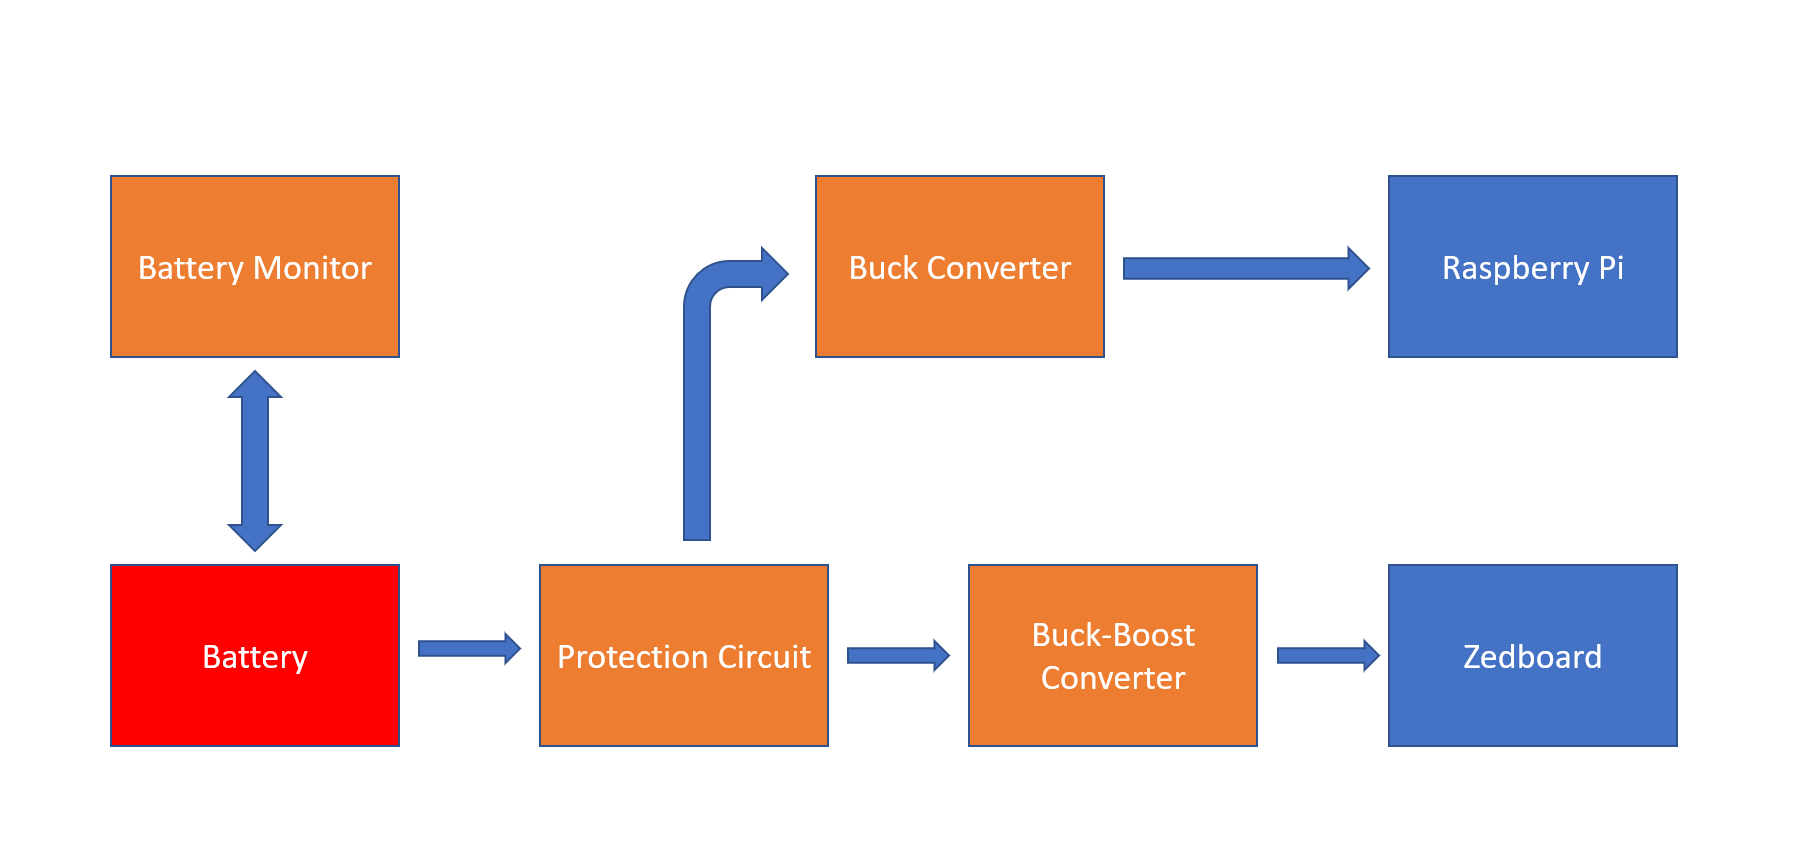
\includegraphics[width=15cm]{img/Power_Diagram.png}
\caption{Original Custom-Designed Computing Power System}
\label{powerdiag}
\end{figure}

Using a custom designed power supply, DC-DC conversion would have been accomplished through use of a buck converter for the 5 V output and a buck-boost converter for the 12 V output.

After designing the system, an alternative commercial power bank was found which fits the project requirements. Said commercial power bank consists of 3 lithium-ion batteries with a combined capacity of 3000mAh in addition to a power management circuit. The power bank provides a 5V/2A USB output port and a 12V/3A output port which are compatible with the Raspberry Pi and the Zedboard respectively. The rated maximum current output from each port is sufficient to simultaneously supply both computation boards, and the battery capacity is rated to provide 3 hours and 45 minutes of operation on a single charge.

\begin{figure}[H]
\centering
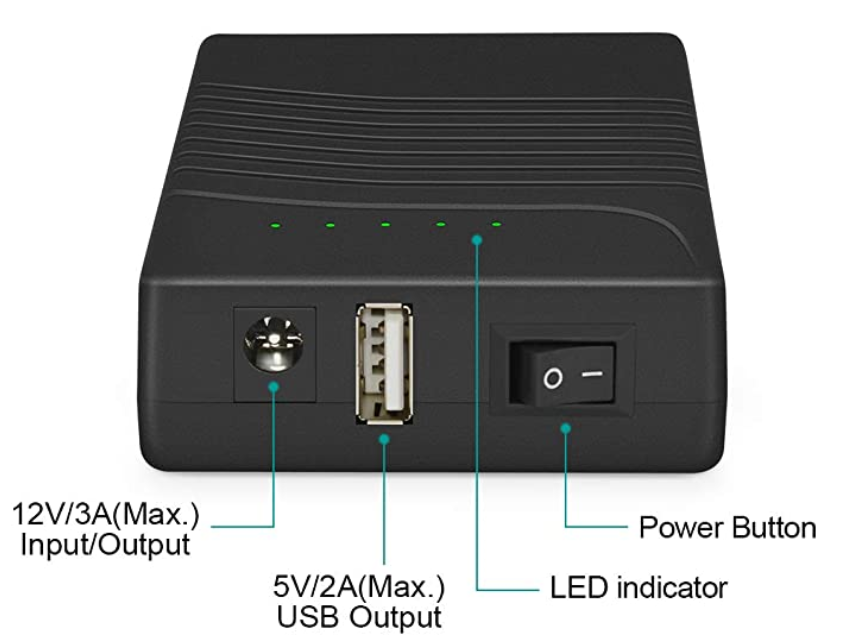
\includegraphics[width=12cm]{img/power_bank.png}
\caption{Commercial Power Bank}
\label{powerbank}
\end{figure}

Ultimately, the commercial power bank was chosen over the custom-designed solution as the commercial system provides all of the requisite functionality at a lower cost and smaller form factor.


\subsection{Multirotor RPAS}\label{multirotor}
The bare-minimum multirotor remote-piloted aerial system (RPAS) consists of a propulsion system, flight controller, speed controllers, battery/fuel, and sensor systems.

\subsubsection{Multirotor Configuration}

A multirotor RPAS (MRPAS) has several common configurations, a tricopter, a quadcopter, and a hexacopter.

\begin{figure}[H]
    \centering
    \begin{subfigure}[b]{0.3\textwidth}
        \centering
        
\includegraphics[scale=0.4]{img/drone_yconfig}
        \caption{Tricopter Y-Configuration}
        \label{fig:tricopter-y}
    \end{subfigure}
    ~
    \begin{subfigure}[b]{0.3\textwidth}
        \centering
        
\includegraphics[scale=0.4]{img/drone_xconfig}
        \caption{Quadcopter X-Configuration}
        \label{fig:quadcopter-x}
    \end{subfigure}
    ~
    \begin{subfigure}[b]{0.3\textwidth}
        \centering
        
\includegraphics[scale=0.4]{img/drone_hexconfig}
        \caption{Hexcopter X-Configuration}
        \label{fig:hexcopter-x}
    \end{subfigure}
    
    \caption{Multirotor RPAS configurations}
    \label{fig:rpas_configs}
\end{figure}

\textbf{Tricopter: }The benefit of a tricopter, as represented in figure \ref{fig:tricopter-y} comes from its fewer required motors and speed controllers,
which means less power draw required to sustain flight. Each arm that is supporting each motor is also wider, at 120 
degrees. This makes the motors and arms of the MRPAS less visible from the mounted camera's point of view. 
However, the downside of a tricopter is that there exists asymmetry of motor torque (figure \ref{fig:tricopter-y-t}) since 
there is an odd number of motors. An additional servo motor is required to control the tail motor which 
complicates the control algorithms for self-stabilizing flight.

\begin{figure}[H]
    \centering
    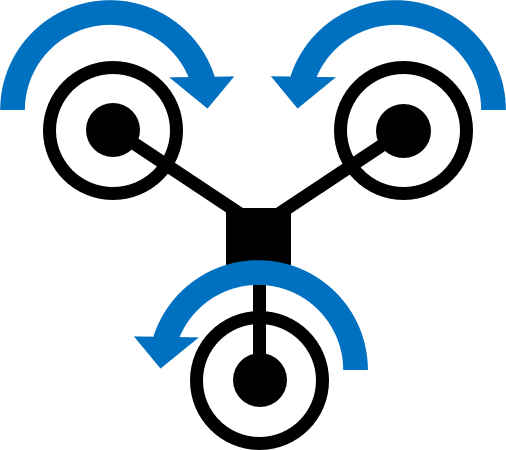
\includegraphics[scale=0.4]{img/drone_yconfigt}
    \caption{Tricopter Y-configuration has non-zero resultant motor torque}
    \label{fig:tricopter-y-t}
\end{figure}

\textbf{Quadcopter X: }
The quadcopter is the most common configuration in consumer multirotor products. The quadcopter is more stable than a tricopter because a quadcopter configuration utilizes four motors (Figure \ref{fig:quadcopter-x-t}). Two of the motors spins  
clockwise and the other two spins counter-clockwise, effectively cancel each other’s undesired torque. 
Applying the same power into each motor allows the MRPAS to hover in place. We can perform 6 degree-of-freedom (DOF) movements by changing a combination of differential thrust to each motor (Figure \ref{fig:rpas_6dof}).

\begin{figure}[H]
    \centering
    
\includegraphics[scale=0.4]{img/drone_xconfigt}
    \caption{Quadcopter X-configuration has zero resultant motor torque}
    \label{fig:quadcopter-x-t}
\end{figure}

\begin{figure}[H]
    \centering
    \begin{subfigure}[b]{0.3\textwidth}
        \centering
        
\includegraphics[scale=0.4]{img/drone_x_pitch}
        \caption{Pitch forward}
        \label{fig:x-pitch}
    \end{subfigure}
    ~
    \begin{subfigure}[b]{0.3\textwidth}
        \centering
        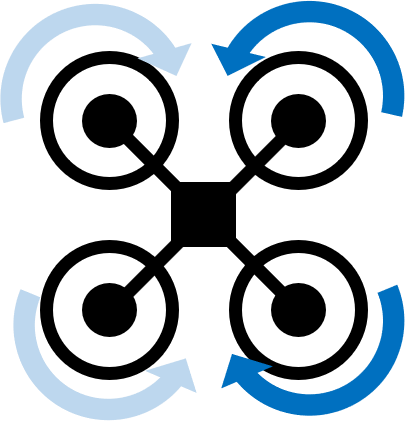
\includegraphics[scale=0.4]{img/drone_x_roll}
        \caption{Roll left}
        \label{fig:x-roll}
    \end{subfigure}
    ~
    \begin{subfigure}[b]{0.3\textwidth}
        \centering
        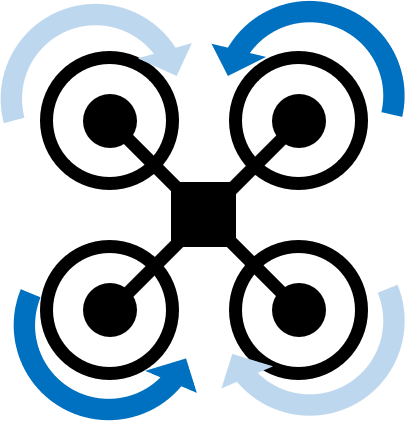
\includegraphics[scale=0.4]{img/drone_x_yaw}
        \caption{Yaw left}
        \label{fig:x-yaw}
    \end{subfigure}
    
    \caption{Using differential thrust to obtain 6-DOF movement. }
    \label{fig:rpas_6dof}
\end{figure}

\textbf{Hexacopter X: }
The hexacopter has all the stability benefits of a copter. In addition, the hexacopter configuration also 
offers redundancy. Up to 2 motors can fail and the MRPAS could still land safely. Due to the added 
propulsion systems (50\% more than the quadcopter configuration), hexacopter can generally lift more 
payload than quadcopters. The downside is that hexacopter configuration builds are more expensive to build, 
operate, and maintain. Upon a crash, due to hexacopter MRPASs extended size and weight cause more injuries 
or collateral damage to nearby equipment.

We choose to pursue with a quadcopter configuration. 
The payload is not too heavy, our target maximum payload weight is less than 500 g (\textbf{NF.DR.1}). The quadcopter configuration is also the most balanced in terms of trade-off between cost and reliability. 

\subsubsection{Air Frame}\label{section:air-frame}

The most common frames available for sale comes in 450 mm motor to motor diagonal span (MMDS). However, 
350mm is also common amongst consumer products such as DJI Phantom. The problem with 350 mm is that it will 
constrain our ability to mount larger hardware such as the computing platform. The 350 mm also limits 
propeller size. On the other hand, the largest quadcopter configuration has an MMDS of 650 mm or 1000 mm 
for extremely large payload capacity. However, these are more commonly used for industrial or military 
applications.

\begin{figure}[H]
    \centering
    \begin{subfigure}[b]{0.33\textwidth}
        \centering
        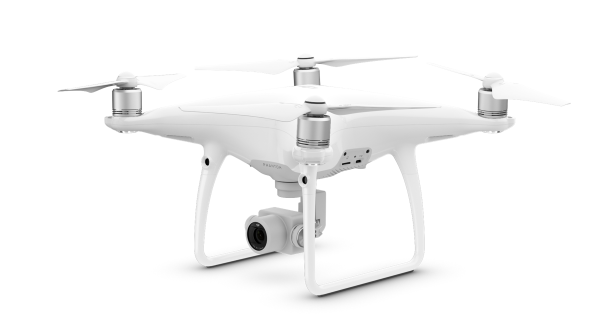
\includegraphics[width=\textwidth]{img/djiphantom4}
        \caption{DJI Phantom 4 (350 mm)}
    \end{subfigure}
    ~
    \begin{subfigure}[b]{0.33\textwidth}
        \centering
        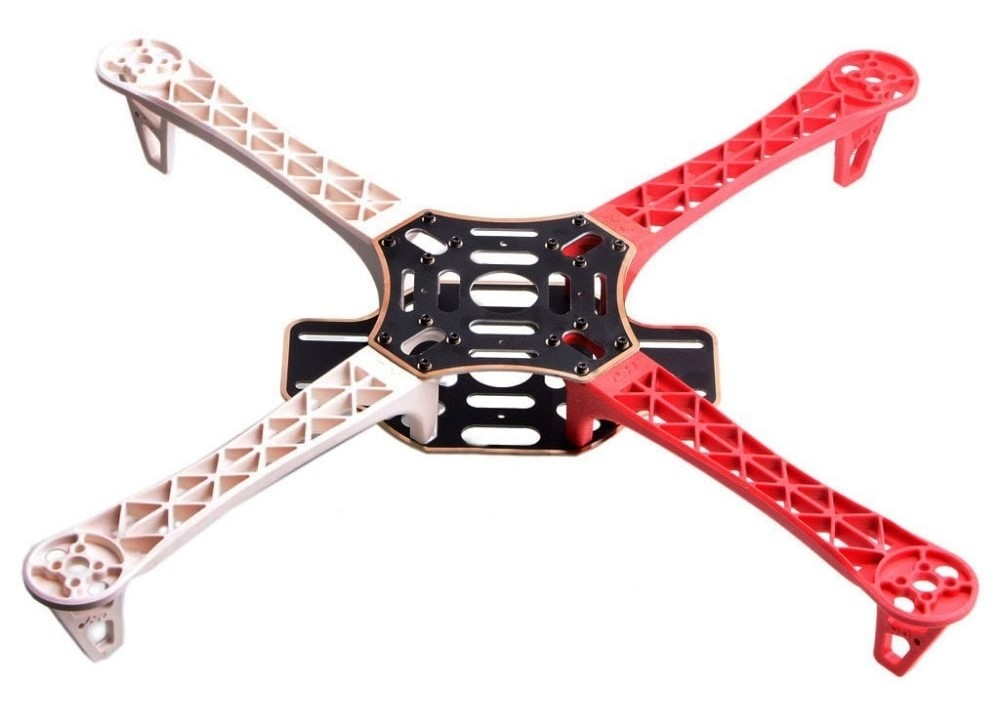
\includegraphics[width=\textwidth]{img/f450frame}
        \caption{Generic DIY frame kit (450 mm)}
    \end{subfigure}
    ~
    \begin{subfigure}[b]{0.33\textwidth}
        \centering
        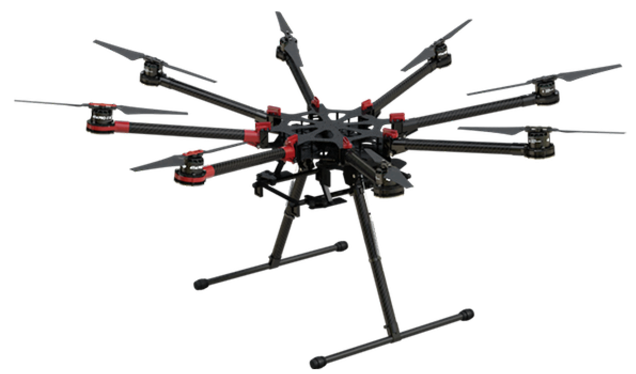
\includegraphics[width=\textwidth]{img/djis1000}
        \caption{DJI Spreadwings S1000 (1000 mm)}
    \end{subfigure}
    
    \caption{Various air frame sizing options. }
    \label{fig:}
\end{figure}

We choose a frame size of 450 mm MMDS that has a good balance between portability and capability. The frame 
can accommodate larger propellers (see in later section XX in propeller size). Furthermore 450 mm are the 
most abundant size on the market for frames because of their versatility and therefore is also less costly 
and easy to repair/replace.

Currently, the \textit{Upgrade F450} for CA\$30.00 and \textit{Diatone Q450} for CA\$20.00 from Banggood are appealing options. They weigh between 300 g to 410 g which is acceptable.

\subsubsection{Propulsion System}

Propulsion system covers the majority of the RPAS parts list and will determine the flight performance of the RPAS. 

\paragraph{Motor Type}

The MRPAs is electrically powered with a battery (DC). Thus, we have two options for motors: DC brushed 
motors and DC brushless motors.

Brushed motors use mechanical brushes in contact with rotor’s commutator to switch polarity to sustain a 
constant rotation, whereas the brushless motors use electronic controllers to switch the polarity in the 
rotor electrically. 

For the flight applications, we choose the brushless DC (BLDC) motors for their extended usable life time. 
BLDC motors are also much more efficient than brushed motors because we do not have to mechanically swap 
the polarity in the motor, which results in excess friction, heat, and potential sparking.

BLDC motors are further broken down into two types: in-runner and out-runner. The in-runner have the rotor 
on the inside and the out-runner has the rotor on the outside. We choose out-runner because they’re 
commonly used for multirotor RPAS. The out-runner also comes with benefits: because the rotor is on the 
outside, heat dissipation is significantly more efficient. Since the rotating mass is further from the 
center of rotation for an out-runner, the rotational inertia helps stabilizing the angular momentum of the 
rotor. Of course, this means that the out-runner has a slower spin-up time than the in-runner, but for a 
multirotor RPAS typically operating in stabilized flight and hover, the agility of an in-runner is not 
practical.

\paragraph{Motor Size and Speed}\label{section:motor-speed}

All BLDC out-runner motors have the same height, and on product pages they are often given the code 22XX to denote their stator size. The design parameter is the radius (XX on the product code). Typically, the larger the stator (radius), the slower it spins given the same voltage. This is a linear relationship described by the motor parameter kV:

$$
\omega_{\mathrm{RPM}} = \mathrm{kV} \times \mathrm{Voltage}
$$

The kV constant is inversely proportional to another motor constant, kT, which models the linear relationship between current and torque:

$$
\tau = \mathrm{kT} \times \mathrm{Current}
$$

The inverse relationship can be shown by equating electrical power into the motor and mechanical power produced by the motor:

$$
\tau\omega_{\mathrm{RPM}} = \mathrm{kV}\mathrm{kT}\times VI
$$

By constraining the electrical power, we can make trade-off between torque and rotation speed.
Air resistance, or “drag” is proportional to speed of an object squared therefore the power required to 
lift increases non-linearly to the force output. As seen in the test data obtained from one manufacturer’s 
datasheet below, using the same propellers we see an increased thrust output from increased voltage (and 
thus current). However, the efficiency, typically measured in g/W decreases. 

Below is a sample set of thrust output using a SunnySky X2216 1250 kV motor using 9.0 inch 5.0\si{\degree} pitch and 10.0 inch 4.7\si{\degree} pitch propellers obtained from vendor website \cite{sunnysky-2216}. 

\begin{table}[H]
    \centering
    \caption{Sample motor test data demonstrates decrease in g/W efficiency as thrust output increases.}
    \label{table:sunnyskyx2216-table}

    \begin{tabular}{lrrrrr}

    \hline
    \textbf{Propeller} & \textbf{Voltage} & \textbf{Current} & \textbf{Pull}  & \textbf{Power Consumption} & \textbf{Efficiency}\\
    & [V] & [A] & [g] & [W] & [g/W] \\
    \hline
     & 10.0 & 16.4 & 940 & 164 & 5.73 \\
    9050 & 11.0 & 19.5 & 1050 & 215 & 4.89 \\
     & 12.0 & 21.5 & 1250 & 258 & 4.84 \\
    \hline
     & 10.0 & 23.5 & 1200 & 235 & 5.10 \\
    1047 & 11.0 & 26.5 & 1350 & 372 & 3.63 \\
     & 12.0 & 30.2 & 1520 & 363 & 4.19 \\
    \hline

    \end{tabular} 
\end{table}

Therefore, it makes sense that we choose larger motors with relatively lower kV constants. Slower motors 
are also safer since there is less angular momentum of the blades. Motors with 800 kV to 1300 kV are 
suitable for our applications and achieve reasonable thrust output with adequate efficiency. 2212, 2214, 
and 2216 stator sizes are suitable in this range of kV.

\paragraph{Propeller Material}

Common RPAS propellers are constructed in either plastic or carbon composite. Plastic is cheap, abundant, 
and relatively flexible. But due to their cheapness, their manufacturing is not as precise which leads to 
aerodynamic inefficiencies. Plastic propellers often require balancing where tape is applied to one of the 
blades such that the weight is balanced---minimizing vibrations. Carbon composite propellers, such as 
carbon fibre blades, are extremely light and subsequently much more expensive. But the carbon composite 
propellers have micro-meter precision manufacturing which provides top efficiency. Carbon composite 
propellers are not flexible and extremely tough. It is more dangerous for persons to be near spinning 
carbon composite propellers due to its sharpness and toughness, and could lead to serious injuries or death.

Due to budget constraint and safety concerns, we choose plastic propellers.

\paragraph{Propeller Size and Pitch}

\textbf{Notation: } Propeller size and pitch is commonly denoted by RRYY where RR is the propeller diameter in inches, and YY is the propeller pitch in degrees. (9050 denotes a propeller with 9 inch diameter, and 5.0 degrees of pitch; 1045 denotes a propeller with 10 inch diameter, and 4.5 degrees of pitch).

\begin{figure}[H]
    \centering
    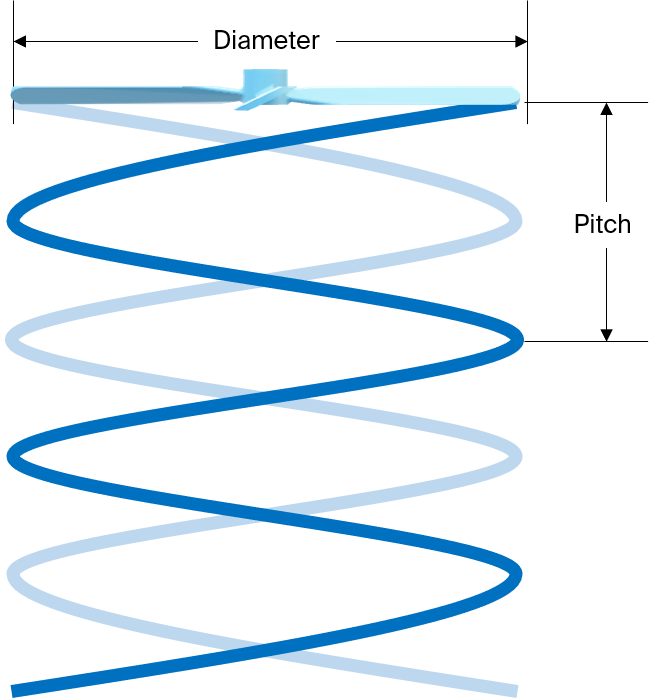
\includegraphics[scale=0.5]{img/proppitch}
    \caption{Diameter and pitch parameters of a propeller}
    \label{fig:propeller}
\end{figure}

To obtain maximum thrust with low speed (low speed is more desirable, as mentioned in Section \ref{section:motor-speed}), we want to choose the biggest possible propeller diameter.

\begin{figure}[H]
    \centering
    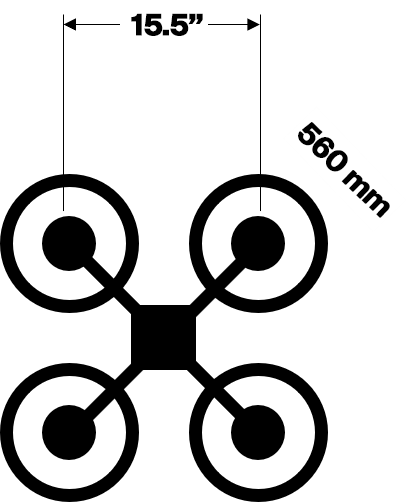
\includegraphics[scale=0.5]{img/framepropsize}
    \caption{Maximum propeller size is determined by the size of the frame.}
    \label{fig:framepropsize}
\end{figure}

As mentioned in Section \ref{section:air-frame}, we choose the 450 mm frames, which means that the motor to motor 
adjacent span (MMAS) is about 12.5 inches. It is safe to provide 1 inch of clearance between propellers, 
therefore the ideal size of propellers we choose is 10 or 11 inches.

Mentioned in  Section \ref{section:motor-speed}, we choose low-speed motors for their efficiencies. And recall that 
given the same power: a slow-speed motor provides inversely proportional high-torque, we choose propellers 
with relatively high pitch (between 3 to 5 degrees) to take advantage of the high-torque output and 
maximize thrust output.

Here is a list of desirable propeller size and pitches: 1030, 1045, 1130, 1145.

\paragraph{Speed Controllers}

The electronic speed controller (ESC) controls the voltage and current supplied to a BLDC motor. All ESCs 
function identically and the design parameters are size/weight, rating, efficiency, and cost.

As shown in Table \label{table:sunnyskyx2216-table} the typical maximum current draw is about 30 A. For a 
safety margin of 10 A, we decided to select ESCs with maximum rating of 40 A. All of below are appealing 
options:

\begin{table}[H]
    \centering
    \caption{ESC Purchasing Options}
    \label{table:esc-table}

    \begin{tabular}{lrrrll}

    \hline
    \textbf{ESC} & \textbf{Rating} & \textbf{Weight} & \textbf{Price}  & & \textbf{Vendor}\\
    & [A] & [g] & [CA\$] & & \\
    \hline
    HAKRC BLHeli Dshot1200 & 35 & 7  & 40.00 & per 4 & Banggood\\
    Racestart RS30A Lite & 30 & 6  & 40.00 & per 4 & Banggood\\
    Racestart SPROG X DShot600 & 35 & 4  & 30.00 & per 4 & Banggood\\
    Skystars Talon32 & 40 & 7  & 12.00 & per 1 & Banggood\\
    \hline

    \end{tabular} 
\end{table}

\subsubsection{Flight Controller}

Flight controller (FC) comes in different tiers differentiated by their price and features. 

The cheapest FC typically only has the bare-minimum features for flight such as accelerometers and 
self-hover functions. These flight controllers are typically designed for acrobatic or basic VLOS 
flying and typically cost CA\$20 to CA\$50. The firmware that runs on these FC are typically 
open-source but nonetheless user-friendly and easily-programmable. Below is a list of FC that falls 
under this tier:

\begin{itemize}[noitemsep,topsep=0pt, parsep=4pt, partopsep=0pt]
    \item F1, F3, F4, F7 FC are minimal in weight and footprint; they are ideal for light-weight operations.\cite{f1fc}
    \item KK 2.15 FC features a built-in display on the board, allowing quick access to flight settings without the need to connect to a computer for reprogramming.
    \item Naze32 FC is reliable with auto-tuning PIDs.
    \item CC3D FC is reliable with auto-tuning PIDs.
\end{itemize}

The next tier of FC have more advanced features such as GPS-hold, autonomous flight, anto-land, 
telemetry, etc. They are designed for more advanced operation. These FCs are more expensive costing 
CA\$50 to CA\$200. However, these FCs have excellent after-sale support for their respective 
manufacturers and documentation is better. The FCs are also rigorously tested in the industry. Along 
with frequent manufacturer firmware updates, the mid-tier FCs are more liable. The downside is that 
they are typically heavier with weather-resistant enclosures and takes up a much larger footprint. 
Below is a list of mid-tier FCs:

\begin{itemize}[noitemsep,topsep=0pt, parsep=4pt, partopsep=0pt]
    \item ArduPilot APM 2.8 is a flight controller using Arduino Mega and supports GPS and telemetry.
    \item Pixhawk PX4 Autopilot features pre-programmable autonomous operations.
    \item DJI Naza M Lite.
\end{itemize}

For the applications we need, we choose ArduPilot APM 2.8 as it is the most flexible option with advanced features at a reasonable price of CA\$75.00. Additionally due to of the low-cost of low-tier FCs, we will also purchase one of Naze32 or CC3D FC as a back-up.

\subsubsection{Radio Systems}

The minimum number of channels required to fly a drone is 4. One for each control: throttle, yaw, 
pitch, and roll. For that reason, we opt for the cheapest radio transmitter (TX) and receiver  (RX) 
combo we find from online vendors. 
The FlySky-FS i6 2.4GHz 6-Channel TX and RX bundle is ideal for our application for its lowcost.
According to FlySky-FS i6 datasheet\cite{flyskyi6} , the radio frequency (RF) peak power is below 20 dBm and still achieves maximum control range of 500 m, and thus satisfies the requirement \textbf{NF.DR.5}.

\subsubsection{Battery}

We choose lithium polymer (Li-Po) batteries because they have the highest energy density (highest 
capacity to weight ratio), and thus perfect for high-power, low-weight applications such as flying. 

Li-Po batteries have mainly three design parameters: configuration, capacity, and discharge rating. 
Configuration is how the Li-Po batteries are wired up: a single-cell Li-Po battery can provide a 
nominal voltage of 3.7 V due to its electrochemistry. Multiple cells can be put in series and the 
voltage adds up: 2S (2 cells in series) batteries have 7.4 V output, 3S batteries have 11.1 V output,
 and 4S batteries have 14.8 V output.

Battery capacity is measured in watt-hours (Wh) or milli-amp-hours (mAh) which is power multiplied by time. A 20 Wh battery can output 20 W for 1 hour. Multiple cells of batteries can be put in parallel and the capacity adds up. 4S2P batteries have 14.8 V ouput but has double the capacity than 4S batteries.

Lastly, the discharge rating is denoted by “C” and indicates the maximum discharge current. A 1,000 
mAh battery with a discharge rating of 20 C can discharge a maximum of 1.0 A $\times$ 20 C = 20 A.

We choose the design parameters for the battery after we have consolidated on rest of the parts for the RPAS since batteries comes in many sizes and configurations, and allows more flexibility.


% Bibliography
\clearpage
\addcontentsline{toc}{section}{References}
\bibliographystyle{ieeetr}
\bibliography{references}

% Appendix (uncomment to enable appendix)
% \clearpage
% \appendix
% \section{Appendix name}\label{appendix:sample-appendix}
% Content here

\end{document}